\Chapter{Útvonalkeresés}
\label{Chap:utvonalkereses}

A fejezet az útvonalkeresésnél alkalmazott módszereket mutatja be.

\section{A waypoint-ok fogalma és jellemzői}

A waypoint a tér egy meghatározott pontja, amely nem látható a játékos számára. A mesterséges intelligencia ezeket használja fel az ellenfelek mozgási útvonalainak meghatározásához. Azért van rájuk szükség, mert a pályán különféle terepakadályok vannak (például falak), különböző játékelemek, amiken nem lehet átmenni, és ezekkel a pontokkal egyértelműen meg lehet határozni a bejárható helyeket.

A waypoint-okhoz rendelhetünk különféle többletinformációkat. Ilyenek lehetnek például, hogy az adott pontban a gépi játékosnak meg kell állnia, le kell guggolnia.

\section{A waypoint-hoz tartozó adatok}

A waypoint-ok pozícióját két dimenziós Descartes koordináta rendszerben $(x, y)$ koordinátákkal adhatjuk meg. Annak ellenére, hogy térben vagyunk, nincs szükség $z$ koordinátára, mert a talaj magassága külön kezelendő, mivel az hatással lesz az ellenfelek viselkedésére. Ennek köszönhetően mindig az adott pálya talajmagasságához tud igazodni, nem szükséges azt külön megadni.

Fontos, hogy a waypoint-nak legyen egy típusa, amely meghatározza, hogy az adott pont milyen szerepet játszik. Ennek segítségével ki lehet számolni, hogy a játékban szereplő karakterek hova mehetnek.

\section{Útvonalkeresés waypoint-ok alapján}

Tegyük fel, hogy a gép létrehoz egy ellenfelet egy véletlenszerű pozícióba. (Ezt a szakzsargonban \textit{spawn}-olásnak hívják.) Az ellenfeleknek az a fő feladatuk, hogy a lehető legrövidebb útvonalon eljussanak a játékoshoz, és megtámadják azt. 

Az útvonalkeresés folyamata a következő fő lépésekből épül fel.
\begin{itemize}
\item A waypoint-ok közül megkeressük az adott karakterhez vagy objektumhoz legközelebbit. Először ezt a pontot kell megközelíteni.
\item A waypoint-ok közül meghatározzuk a célponthoz legközelebbit, ez lesz majd a célpont.
\item A pont adott, kis sugarú környezetét elérve A*-algoritmus segítségével meghatározzuk a legrövidebb útvonalat.
\item A célpontot elérve már csak az adott karakterhez vagy objektumhoz kell egyenes úton eljutni.
\end{itemize}

% TODO: Készíteni egy demo-t az A*-algoritmushoz, és megnézni, hogy a legközelebbi pontok keresése pontosan hogy nézne ki, és egyáltalán kell-e hozzá külön heurisztika.

\begin{algorithm}[H]
  \KwData{ \\
    $S \in \mathbb{R}^2$, a kezdőpont, aktuális pozíció \\
    $W = \{w_i | w_i \in \mathbb{R}^2\}$, a waypoint-ok halmaza
  }
  \KwResult{ \\
    $T \in \mathbb{R}^2$, az elérendő pont,
  }
  $\displaystyle T = \min_{||w_i - S||_2} w_i$
  \caption{A legközelebbi pont megkeresése}
\end{algorithm} 

% TODO: Itt az algoritmust még pontosítani kellene, illetve megnézni, hogy az A*-ot nem elegendő-e közvetlenül alkalmazni!

\begin{algorithm}[H]
 \KwData{Waypoint vegso\_pont\;\\ Vec2 legkozelebbi\_pont\;\\double pont\_tav, temp, x\_tav, y\_tav\;\\ float x, y\; }
 \KwResult{Legközelebbi pont x és y koordinátája}
 pont\_tav := 100000\;
 \For {Waypoint pont : waypointokon}{
 	x := pont.x;\\
	y := pont.y;\\
	x\_tav := |(x – jelenlegi\_xpoz)|;\\
	y\_tav := |(y – jelenlegi\_ypoz)|;\\
	temp := sqrtf(x\_tav * x\_tav +  y\_tav * y\_tav)\;
  \If{temp < pont\_tav}{
   		pont\_tav := temp;\\
		vegso\_pont := pont\;
   }
   legkozelebbi\_pont.x := vegso\_pont.x;\\
   legkozelebbi\_pont.y := vegso\_pont.y\;
 }
 \caption{A legközelebbi pont megkeresése}
\end{algorithm} 

\section{Az A*-algoritmus}

% TODO: Keresni A*-algoritmusos irodalmat/hivatkozást.

Ezt az algoritmust a hatékonysága miatt gyakran használják gráfokban való legrövidebb útvonalak kereséséhez. Bemenetként a gráf két pontját adjuk meg, eredményül pedig az ezek között lévő legrövidebb útvonalat várjuk.

A gyakorlati problémák jelentős részében nem közvetlenül egy gráf áll a rendelkezésünkre. Ahhoz, hogy az A* algoritmust mégis használni tudjuk, a bejárandó területet (amelyben a legrövidebb útvonalat keressük) egy ráccsal közelíthetjük. Ez a rácsos kialakítás több szempontból is előnyös. A pontok minden esetben egymástól egyenlő távolságra helyezkednek el, így ezeket nem kell számolni. Továbbá ha csak a bejárható helyekre helyeznénk pontokat, külön olyan algoritmusra lenne szükség, amely meghatározza azt, hogy melyik pontból melyikbe haladhatunk. A gráf összes csomópontjának és élének a tárolására szükség lenne, amely indokolatlanul sok adat kezelését jelentené. Jelen esetben egy egyenközű rácsot alkalmazva a kereséshez használt gráfhoz, elegendő csak megadni a rácspontokban, hogy az adott pont bejárható vagy nem.

Négyzetrács esetében eldöntendő kérdés, hogy az átlók mentén haladhatunk-e.

% TODO: Itt melyik eset, és miért előnyös? Lehet haladni átlóban?

Az algoritmus végrehajtásához listát kell vezetni azon pontokról amiket még nem jártunk be, illetve azokról is, amelyeket bejártunk, ezeket hívjuk nyitott (Open) illetve zár t (Closed) csomópont listáknak. A nyitott csomópontok listája az, amelyek vizsgálatára még a későbbiekben szükség lehet, a zárt csomópont lista pedig a már vizsgált pontok halmaza.

% TODO: Ide kellene hivatkozás, hogy a nyitott és a zárt csomópontok listája honnan jött!

A csomópontokhoz tárolni kell az addig bejárt távolságot, illetve le kell tárolni egy prioritás változót is, amiben az eddig megtett út, és a még hátralevő út távolságainak összege található. Fontos ugyanis az algoritmus működése szempontjából az eddig megtett, és a hátralévő út, ugyanis ezekből az adatokból számolja ki egy adott pont prioritását (kezdőponttól való táv + célponttól való táv), és így dönti el milyen pontokat részesítsen előnyben. A prioritás minél kisebb érték, annál jobb, tehát arra kell tovább indulni.

Az A* algoritmus leírása pszeudokóddal:
A célpontot jelöljük goal\_node-dal, a kezdőpontot pedig start\_node-dal.

% TODO: A szöveges leírásokat ahol lehet tömörebb, képletes formában kellene megadni!

% TODO: Ezt, vagy valami hasonlót be kellene hivatkozni: http://mat.uab.cat/~alseda/MasterOpt/AStar-Algorithm.pdf

\begin{verbatim}
1.Helyezük a start_node-ot az Open listába. f(start_node)=h(start_node)
2.Amíg az Open lista nem üres
3.	Vegyük a az Open listából azt a node-ot, amely a legkisebb költségű
4.		f(current_node) = g(current_node) + h(current_node)
5.	ha current_node a célpont, megtaláltuk a megoldást; break
6.	Generáljunk minden állapothoz successor_node-ot, ami a 
		current_node-ból származik
7.	ciklus minden current_node successor_node-ján
8.		Állítsuk be a successor_current_költséget, amely g(current_node) 
				+ w(current_node, successor_node)
9.		ha successor_node az Open listában van
10.			ha g(successor_node) <= successor_current_költség ugrás 19-re
11.			különben ha successor_node a Closed listában van
12.			ha g(successor_node) <= successor_current_költség ugrás 19-re
13.			Mozgassuk successor_node-ot a Closed listából az Open listába
14.		    különben
15.			Adjuk hozzá successor_node-ot az Open listához
16.			Állítsuk a h(successor_node)-ot hogy megkapjuk a heurisztikus 
				távolságot a célig
17.		Legyen egyenlő g(successor_node) a successor_current_költséggel
18.		Állítsuk be node_successor szülőjét current_node-nak
19.	Adjuk hozzá a current_node-ot a Closed listához
20.ha(current_node != goal_node) lépjünk ki a következővel: 
						(az Open lista üres)
\end{verbatim}

\section{A keresési algoritmus implementációja}

A program a játéktér alapját képző domborzatot, egy képből olvassa be. Ez a magasságmező, ahol egy adott pont magasságát a világossága határozza meg, minél világosabb, annál magasabb pontot jelent a domborzaton, így 256 féle magasság lehetséges, ami az aktuális változathoz megfelelő felbontásnak bizonyult. 

A játékteret úgy érdemes kialakítani, hogy jelentős része (körülbelül 95\%) bejárható legyen.

% TODO: A felbontást még érdemes lenne részletezni, mert nem tünik kézenfekvőnek, hogy pont 384x384 legyen.

A magasságmezőhöz tartozó kép felbontása $384 \times 384$ pixel, amely a térkép megfelelő részletességű megjelenítése miatt ennyi. A waypoint-ok meghatározására több lehetőség is van.

Az egyik lehetőség, ha minden pixelhez rendelünk egy pontot. Ez olyan szempontból lehet előny, hogy pontosabban meg van határozva az összes pont amelyre léphet az ellenfél. Hátránya viszont, hogy ez nagyon sok számításigény, és fölösleges is minden pixelre egy waypoint.

A másik lehetőség, ha 8 pixelenként határozunk meg egy waypoint-ot, ami 48x48-as felbontást eredményez. Azért pont erre az értékre esett a választásom, mert ez nagyban gyorsítja a számításokat, viszont még nem megy a bejárható területek rovására, megfelelően pontos. Ez kevesebb memória igényt jelent, és mivel kevesebb adattal is kell számolni, kevésbé terheli a processzort is. Ez látható \aref{fig:diagram_utvonal} ábrán.

% TODO: Ez az ábra így nagyon apróbetűs. Érdemes lehet egy kisebb felbontású, inkább sraffozott, vagy szinezett megoldást választani.

\begin{figure}[h]
\centering
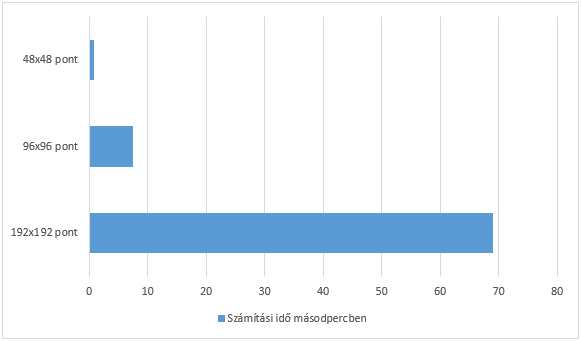
\includegraphics[scale=0.9]{kepek/utvonal_szamitas_diagram_waypointokra.png}
\caption{Számításigény a felbontás és idő függvényében}
\label{fig:diagram_utvonal}
\end{figure}

Első lépésként, létre kell hozni a waypoint hálót, amiken a mesterséges intelligencia végig fog menni, elkerülvén hogy átmenjen a tereptárgyakon, falakon. Ezek a pontok 8 pixelenként, függetlenül az adott pixel színétől meghatározásra kerülnek, viszont a típusa az adott pixel színének megfelelően lesz beállítva. Ahogy \aref{fig:kuszobertek}-as ábrán is látható, a például egy pont színéből 50-nél nagyobb érték jön ki, akkor a pont típusa zártra állítódik, így ebbe az irányba nem lesz lehetséges a továbbhaladás. \aref{fig:mi_printscreen}  képen „.”-al a bejárható terület, „X”-el a falak, „S”-el az indulópont, „F”-el a célpont, „R”-el a legrövidebb útvonal van jelölve.

\begin{figure}[h]
\centering
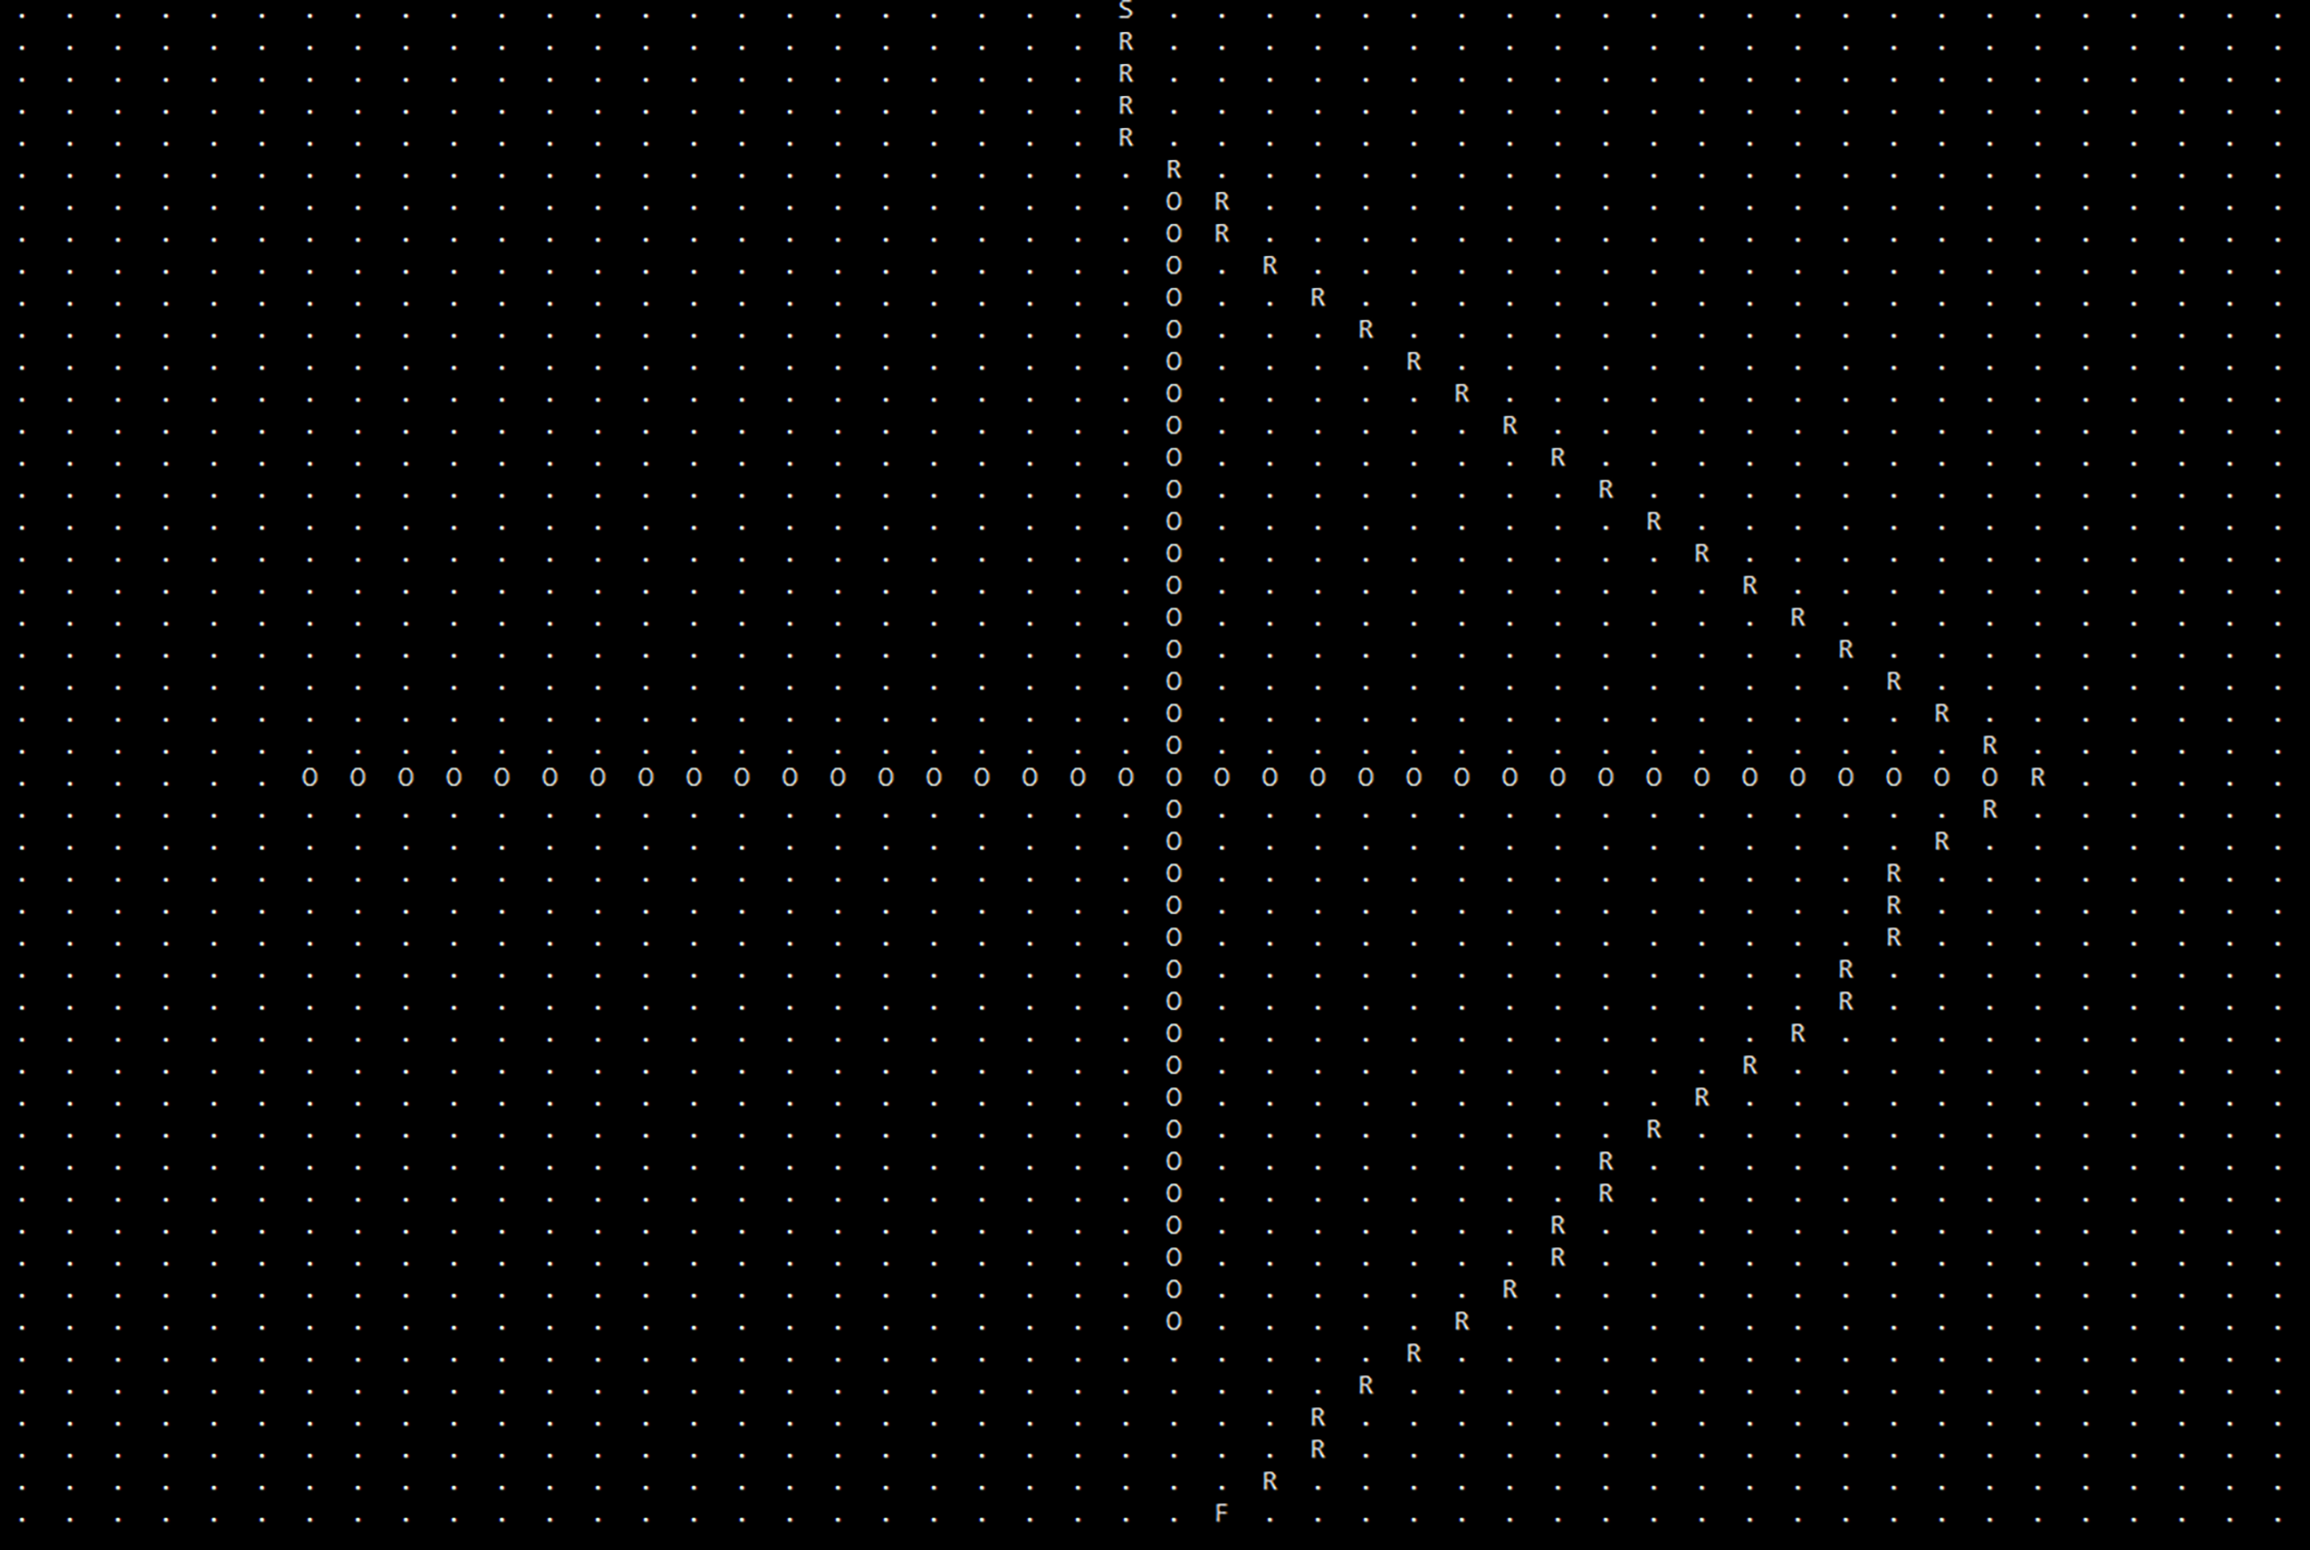
\includegraphics[scale=0.22]{kepek/mi_printscreen.png}
\caption{Útvonal meghatározó algoritmus működése}
\label{fig:mi_printscreen}
\end{figure}

A képen még csak statikusan vannak megadva a falak, de mint ahogy fentebb olvasható, a játékon belül a beolvasott magasságmező pontbeli értékei határozzák meg azt. Erre azért van szükség, mert így lehet megoldani azt, hogy a mesterséges intelligencia alkalmazkodjon a környezetéhez. Ha a pályától függetlenül, statikusan lenne az összes waypoint típusa meghatározva, akkor ha a játékos más pályát rajzol, a pontok típusai nem illeszkednének az elrendezésre. Ezt a módszert alkalmazva, meg lehet adni, hogy egy bizonyos magasságnál csak másszon, vagy ugorjon, vagy bármilyen más tevékenységet végezzen. Ez egy fontos tulajdonsága a játéknak, mert azt úgy terveztem, hogy a felhasználó tetszőleges raszteres rajzprogram segítségével elkészíthesse a térképet, ne legyen hozzá szükség speciális szerkesztőeszközre. A program a bejárható teret ebből képes közvetlenül meghatározni, be tudja állítani, hogy a falakon a játékos ne tudjon átmenni, a meredek lejtőkről visszacsússzon.

\begin{figure}[h]
\centering
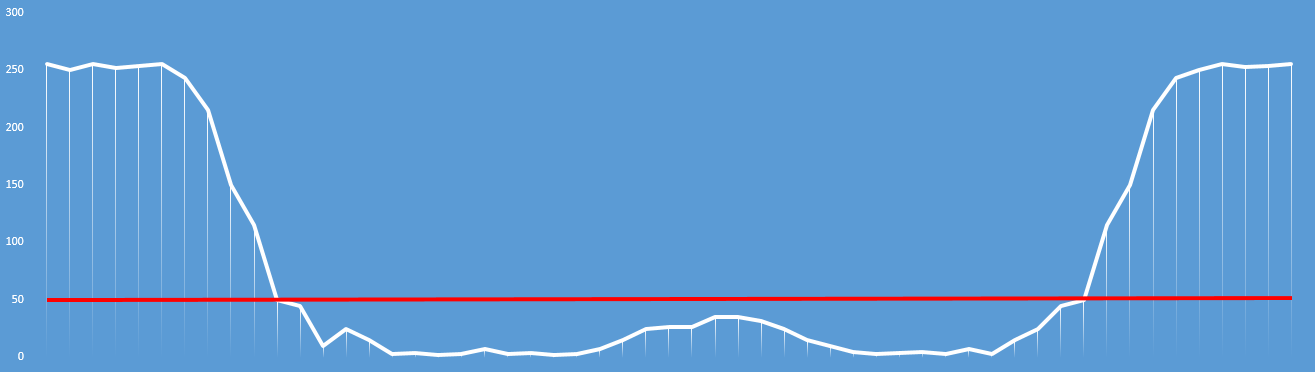
\includegraphics[scale=0.42]{kepek/magassagmezo_kuszobertek_diagram.png}
\caption{Küszöbérték a még bejárható terület meghatározásához}
\label{fig:kuszobertek}
\end{figure}

% TODO: Érdemes lenne a gradienses küszöböléses megoldást is megnézni! (Élkiemelést is lehet hozzá használni.)

De a küszöbérték megadása nem mindig elegendő, ugyanis lehetnek olyan helyek a pályán, amelyek fal magasságúak, de bejárhatók, mert alacsony meredekségű emelkedő vezet fel oda. Ezt a problémát gradiens számítással lehet megoldani, ezzel van megoldva az is, hogy a játékos ne tudjon kimenni a játéktérből. Ahol túl nagy a meredekség, ott a waypoint típusát nem bejárhatóra kell állítani.

A pontok típusának a pálya alapján legenerálása után, az A*-algoritmus segítségével meghatározza a program a legrövidebb útvonalat a cél waypointig, természetesen a pontok típusait figyelembe véve. Ezt másodpercenként legalább 15x újra kell számolni, ugyanis a játékos mozog, és a cél waypoint mindig a játékoshoz legközelebb eső pont, ami ezzel együtt változik.
